\documentclass[10pt]{beamer}
\usepackage[english]{babel}
\usepackage[utf8]{inputenc}
\usepackage[T1]{fontenc}
\usepackage{helvet}
\usepackage{lipsum}  
\usepackage{graphicx, subfigure}


%-------------------------------------------------------
% INFORMATION IN THE TITLE PAGE
%-------------------------------------------------------

\newcommand{\cstitle}{\textbf{Neoantigen Detection Using Transformers and Transfer Learning in the Cancer Immunology Context}
\subtitle[]{Tésis de doctorado}}
\newcommand{\cscourseCode}{PACBB Doctoral Consortium}
\newcommand{\csauthor}{MSc. Vicente Machaca Arceda}
\institute[UNSA]{Universidad La Salle}
\newcommand{\csemail}{vmachaca@utec.edu.pe}
\newcommand{\instituteabr}{UTEC}
\newcommand{\nameUp}{}
\date{2023}
\title[\cscourseCode]{\cstitle}
\author{\csauthor}
%%%%%%%%%%%%%%%%%

%-------------------------------------------------------
% CHOOSE THE THEME
%-------------------------------------------------------
\def\mycmd{0} % UNSA
\def\mycmd{1} % SALLE
%\def\mycmd{2} % UTEC
%-------------------------------------------------------

\if\mycmd0
\usepackage{csformat}
\newcommand{\chref}[3][blue]{\href{#2}{\color{#1}{#3}}}%

\fi

\if\mycmd1
\usetheme[]{Feather}
\newcommand{\chref}[2]{	\href{#1}{{\usebeamercolor[bg]{Feather}#2}} }
\fi

\if\mycmd2
\usetheme{UTEC2020}	
\newcommand{\chref}[3][blue]{\href{#2}{\color{#1}{#3}}}%
\fi

\newcommand{\1}{
	\setbeamertemplate{background}{
		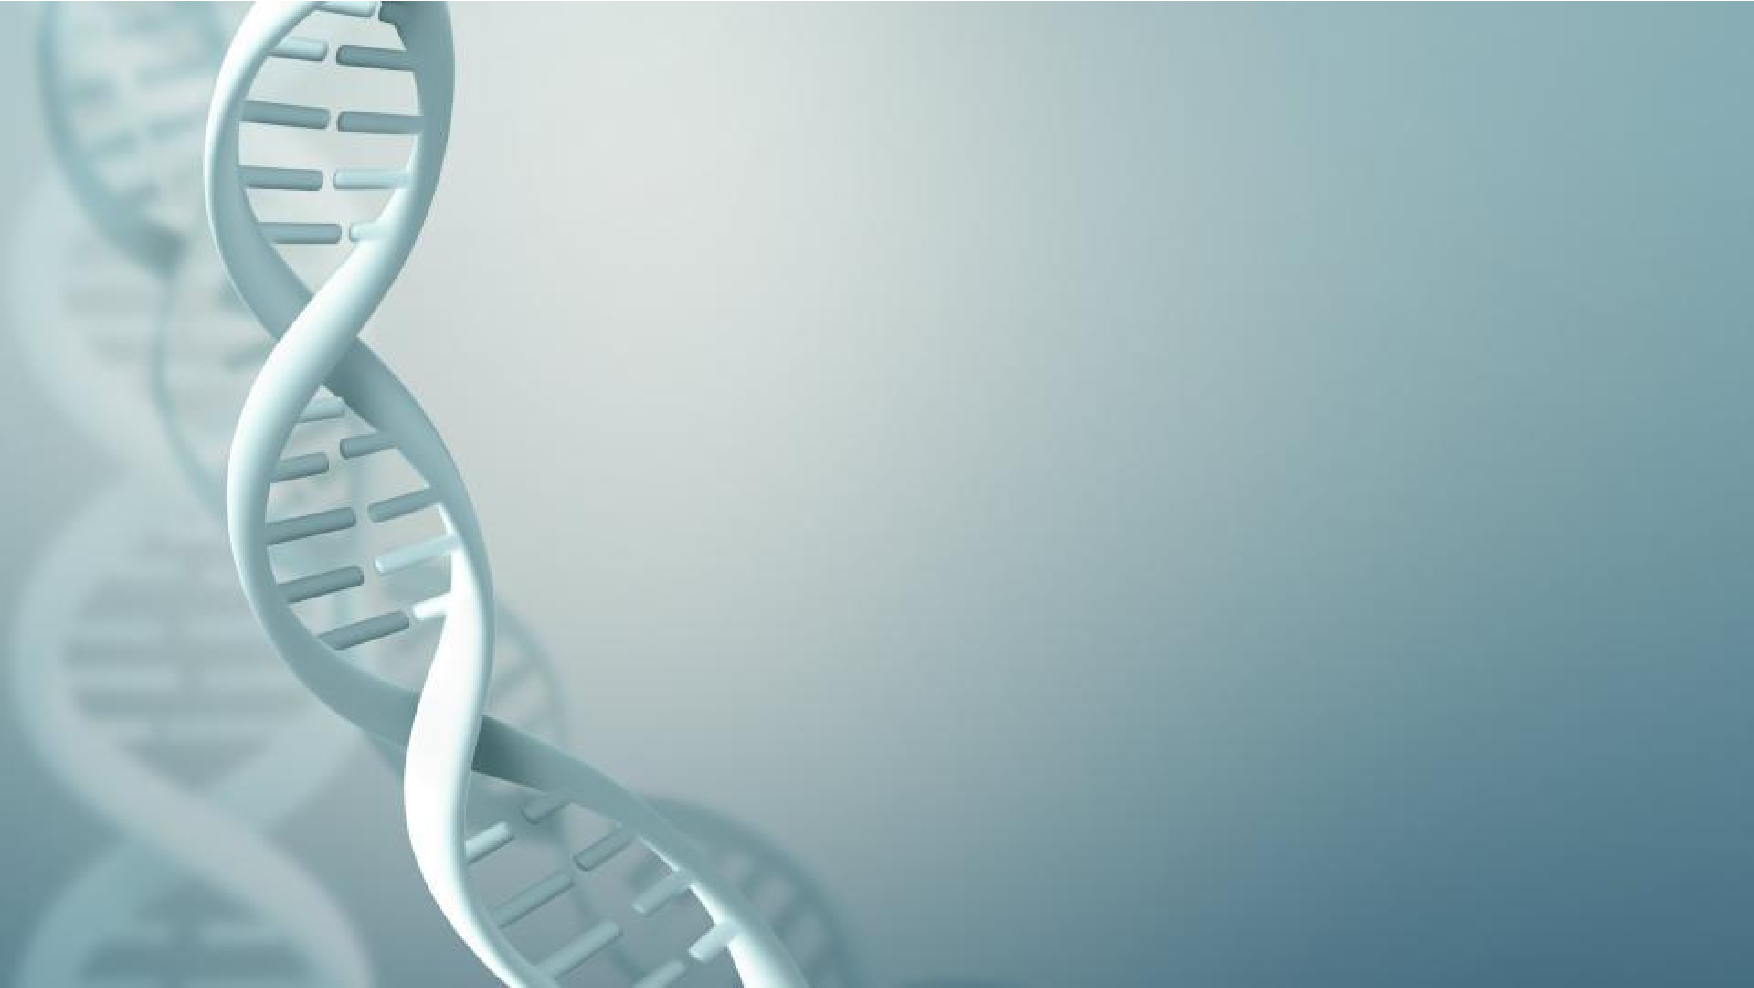
\includegraphics[width=\paperwidth,height=\paperheight]{img/1}
		\tikz[overlay] \fill[fill opacity=0.75,fill=white] (0,0) rectangle (-\paperwidth,\paperheight);
	}
}



%-------------------------------------------------------
% THE BODY OF THE PRESENTATION
%-------------------------------------------------------

\begin{document}
	
	
	\AtBeginSubsection[]
	{
		\begin{frame}
			\frametitle{Content}
			\tableofcontents[currentsubsection]
		\end{frame}
	}
	
	
	%-------------------------------------------------------
	% THE TITLEPAGE
	%-------------------------------------------------------
	
	\if\mycmd0
	\maketitle
	\fi
	
	\if\mycmd1 % MY THEME
	\1{
		\begin{frame}[plain,noframenumbering] 
			\titlepage 
	\end{frame}}
	\fi
	
	\if\mycmd2
	\begin{frame}
		\titlepage
	\end{frame}
	\fi
	%-------------------------------------------------------
	%-------------------------------------------------------


%-------------------------------------------------------
%-------------------------------------------------------
\begin{frame}{Content}
	\tableofcontents
\end{frame}
%-------------------------------------------------------
%-------------------------------------------------------


%%%%%%%%%%%%%%%%%%%%%%%%%%%%%%%%%%%%%%%%%%%%%%%%%%%%%%%%%%%%%%%%%%%%%%%%%%%%%%%%%%%%%%%%%%%%%%%%%%%%%%%%%%%%%%%%
%%%%%%%%%%%%%%%%%%%%%%%%%%%%%%%%%%%%%%%%%%%%%%%%%%%%%%%%%%%%%%%%%%%%%%%%%%%%%%%%%%%%%%%%%%%%%%%%%%%%%%%%%%%%%%%%
%%%%%%%%%%%%%%%%%%%%%%%%%%%%%%%%%%%%%%%%%%%%%%%%%%%%%%%%%%%%%%%%%%%%%%%%%%%%%%%%%%%%%%%%%%%%%%%%%%%%%%%%%%%%%%%%
\section{Introduction}
%%%%%%%%%%%%%%%%%%%%%%%%%%%%%%%%%%%%%%%%%%%%%%%%%%%%%%%%%%%%%%%%%%%%%%%%%%%%%%%%%%%%%%%%%%%%%%%%%%%%%%%%%%%%%%%%
%%%%%%%%%%%%%%%%%%%%%%%%%%%%%%%%%%%%%%%%%%%%%%%%%%%%%%%%%%%%%%%%%%%%%%%%%%%%%%%%%%%%%%%%%%%%%%%%%%%%%%%%%%%%%%%%
%%%%%%%%%%%%%%%%%%%%%%%%%%%%%%%%%%%%%%%%%%%%%%%%%%%%%%%%%%%%%%%%%%%%%%%%%%%%%%%%%%%%%%%%%%%%%%%%%%%%%%%%%%%%%%%%


%%%%%%%%%%%%%%%%%%%%%%%%%%%%%%%%%%%%%%%%%%%%%%%%%%%%%%%%%%%%%%%%%%%%%%%%%%%%%%%%%%%%%%%%%%%%%%%%%%%%%%%%%%%%%%%%
%%%%%%%%%%%%%%%%%%%%%%%%%%%%%%%%%%%%%%%%%%%%%%%%%%%%%%%%%%%%%%%%%%%%%%%%%%%%%%%%%%%%%%%%%%%%%%%%%%%%%%%%%%%%%%%%
%%%%%%%%%%%%%%%%%%%%%%%%%%%%%%%%%%%%%%%%%%%%%%%%%%%%%%%%%%%%%%%%%%%%%%%%%%%%%%%%%%%%%%%%%%%%%%%%%%%%%%%%%%%%%%%%
\subsection{Immunotherapy to Treat Cancer}
%%%%%%%%%%%%%%%%%%%%%%%%%%%%%%%%%%%%%%%%%%%%%%%%%%%%%%%%%%%%%%%%%%%%%%%%%%%%%%%%%%%%%%%%%%%%%%%%%%%%%%%%%%%%%%%%
%%%%%%%%%%%%%%%%%%%%%%%%%%%%%%%%%%%%%%%%%%%%%%%%%%%%%%%%%%%%%%%%%%%%%%%%%%%%%%%%%%%%%%%%%%%%%%%%%%%%%%%%%%%%%%%%
%%%%%%%%%%%%%%%%%%%%%%%%%%%%%%%%%%%%%%%%%%%%%%%%%%%%%%%%%%%%%%%%%%%%%%%%%%%%%%%%%%%%%%%%%%%%%%%%%%%%%%%%%%%%%%%%

%-------------------------------------------------------
%-------------------------------------------------------
\begin{frame}{Immunotherapy to Treat Cancer}{}		
	Immunotherapy is a type of cancer treatment that helps your immune system fight cancer \cite{inmunoterapy2022}.
	
	\begin{figure}
		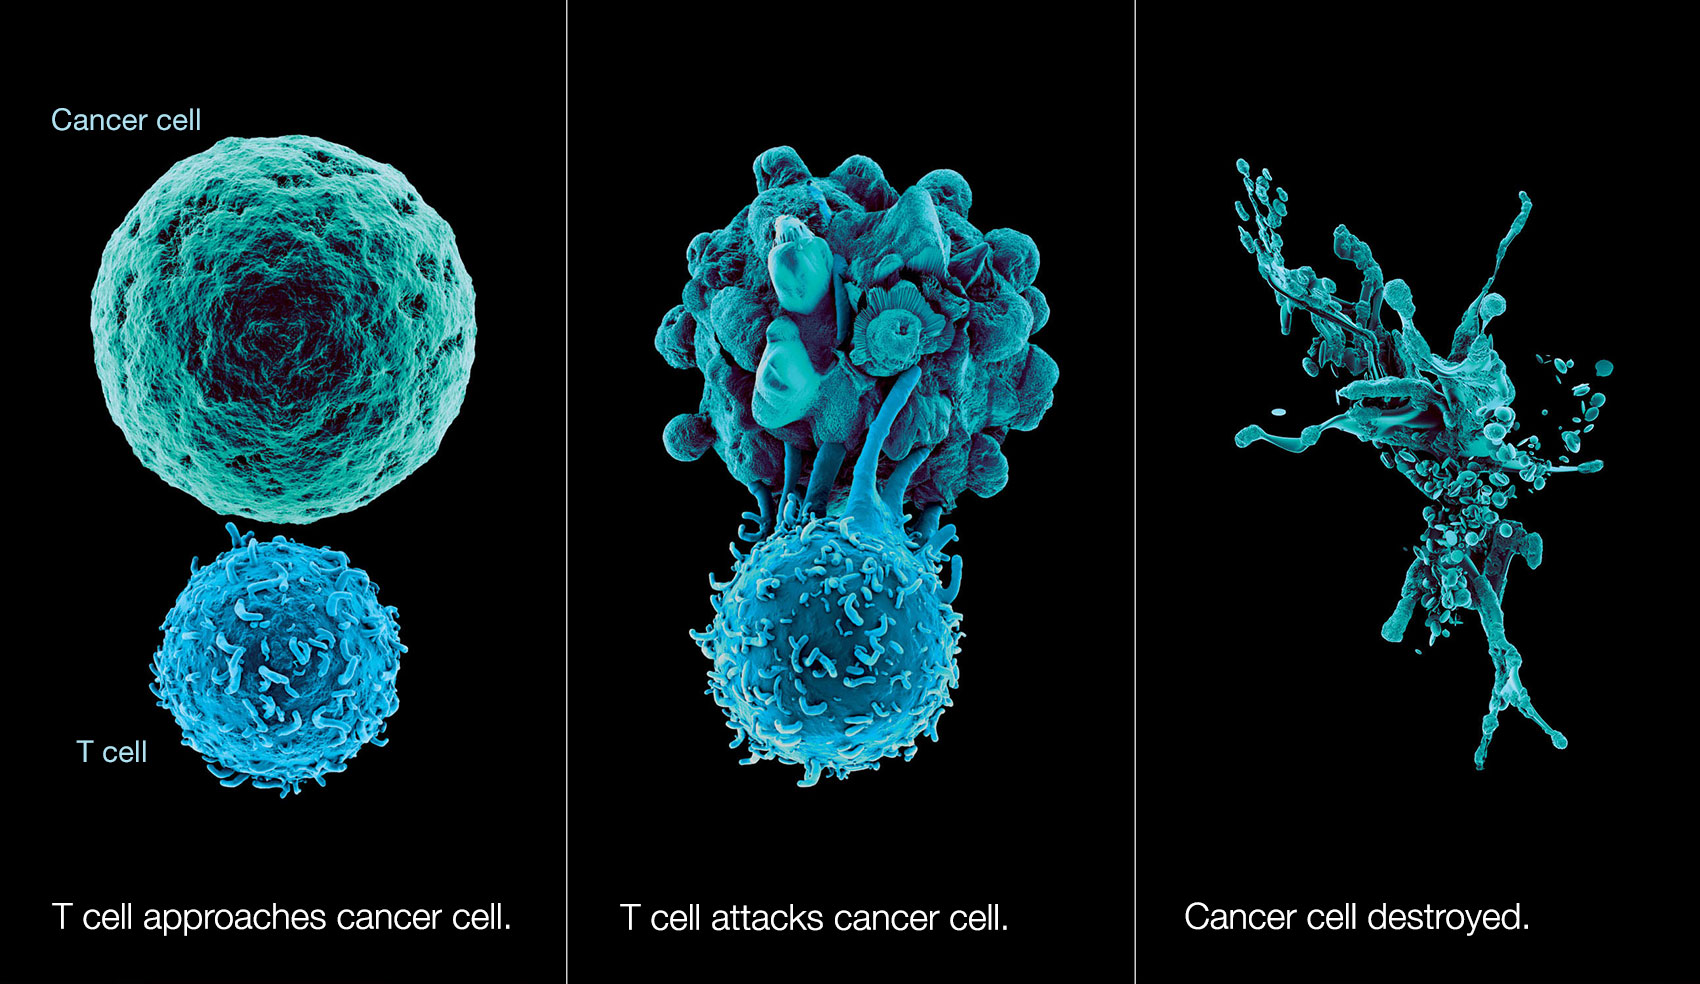
\includegraphics[width=0.85\textwidth]{img/neoantigen/tcell}
		\caption{Example of how a T cell attack a cancer cell \cite{nortshore2022}.}
	\end{figure}		
\end{frame}
%-------------------------------------------------------
%-------------------------------------------------------

%-------------------------------------------------------
%-------------------------------------------------------
\begin{frame}{Immunotherapy to Treat Cancer}{Neoantigen}		
	\begin{block}{Neoantigen}
		A new protein that forms on cancer cells when certain mutations occur in tumor DNA. Neoantigens used in vaccines and other types of immunotherapy are being studied in the treatment of many types of cancer \cite{NCIdictionary2022, borden2022cancer}.
	\end{block} 
	\begin{block}{}
		Currently, there is a lot of methods to detect neoantigens; however, only a small number of them manage to stimulate the immune system \cite{chen2021challenges, hao2021improvement}.
	\end{block}
\end{frame}
%-------------------------------------------------------
%-------------------------------------------------------


%-------------------------------------------------------
%-------------------------------------------------------
\begin{frame}{Immunotherapy for Cancer}{Personalized Vaccines}	
	\begin{figure}
		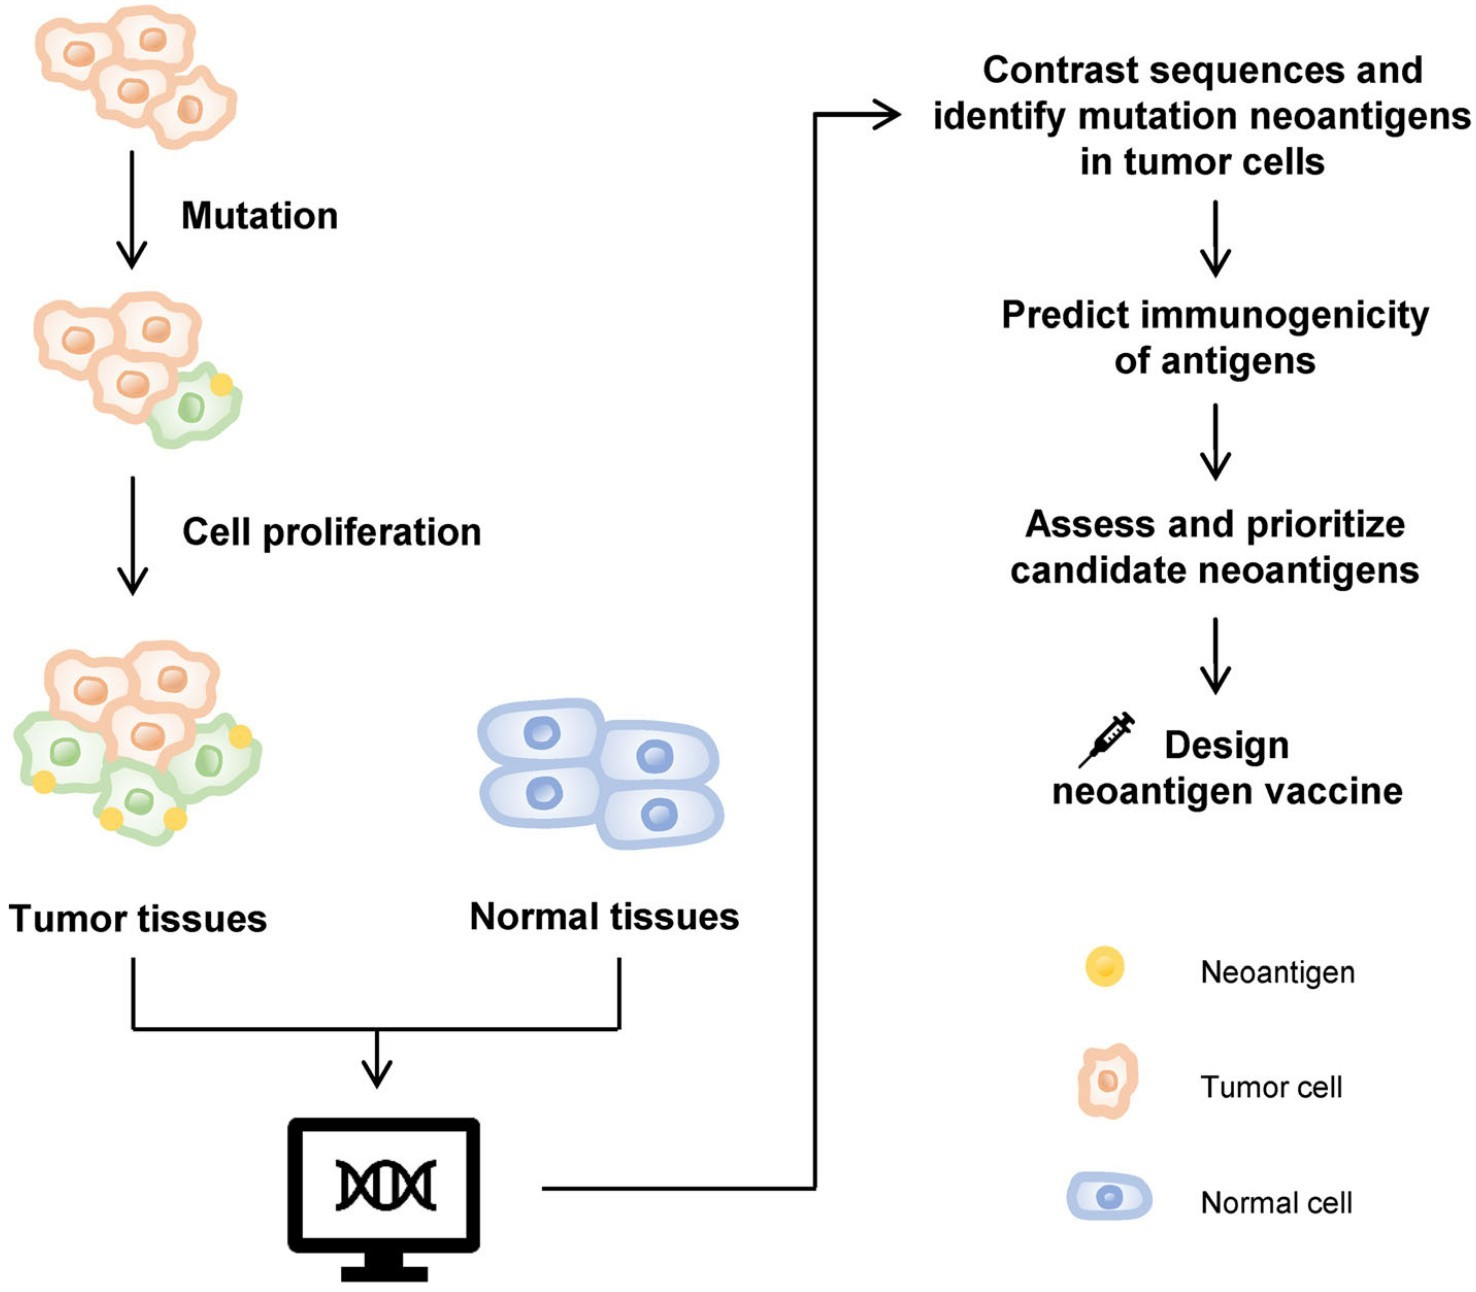
\includegraphics[width=0.6\textwidth]{img/neoantigen/process}
		\caption{Personalized vaccines process for Cancer \cite{peng2019neoantigen}.}
	\end{figure}		
\end{frame}
%-------------------------------------------------------
%-------------------------------------------------------



%-------------------------------------------------------
%-------------------------------------------------------
\begin{frame}{pMHC binding and presentation prediction}{}		
	\begin{figure}[H]
		\centering
		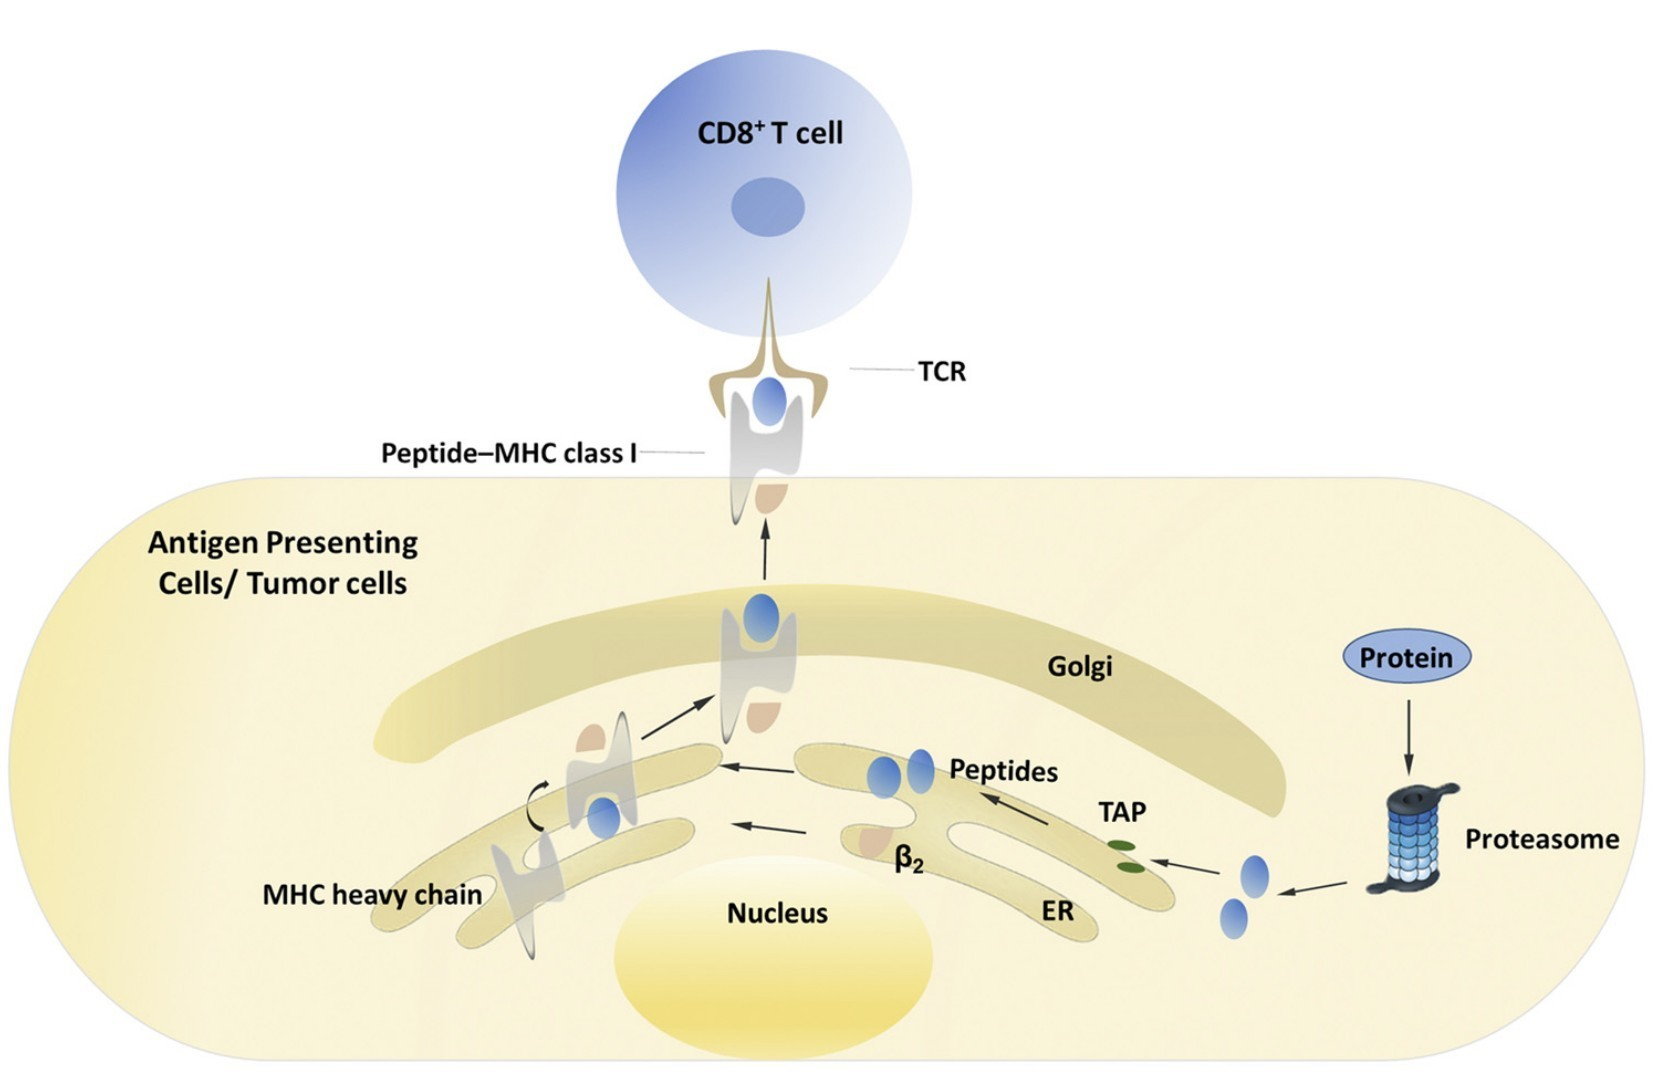
\includegraphics[width=0.9\textwidth]{img/neoantigen/mhc1.jpg}
		\caption{pMHC presentation process in MHC class I \cite{zhang2019application}.}
		\label{fig:mhc1}
	\end{figure}	
\end{frame}
%-------------------------------------------------------
%-------------------------------------------------------

%%%%%%%%%%%%%%%%%%%%%%%%%%%%%%%%%%%%%%%%%%%%%%%%%%%%%%%%%%%%%%%%%%%%%%%%%%%%%%%%%%%%%%%%%%%%%%%%%%%%%%%%%%%%%%%%
%%%%%%%%%%%%%%%%%%%%%%%%%%%%%%%%%%%%%%%%%%%%%%%%%%%%%%%%%%%%%%%%%%%%%%%%%%%%%%%%%%%%%%%%%%%%%%%%%%%%%%%%%%%%%%%%
%%%%%%%%%%%%%%%%%%%%%%%%%%%%%%%%%%%%%%%%%%%%%%%%%%%%%%%%%%%%%%%%%%%%%%%%%%%%%%%%%%%%%%%%%%%%%%%%%%%%%%%%%%%%%%%%
\subsection{Problem}
%%%%%%%%%%%%%%%%%%%%%%%%%%%%%%%%%%%%%%%%%%%%%%%%%%%%%%%%%%%%%%%%%%%%%%%%%%%%%%%%%%%%%%%%%%%%%%%%%%%%%%%%%%%%%%%%
%%%%%%%%%%%%%%%%%%%%%%%%%%%%%%%%%%%%%%%%%%%%%%%%%%%%%%%%%%%%%%%%%%%%%%%%%%%%%%%%%%%%%%%%%%%%%%%%%%%%%%%%%%%%%%%%
%%%%%%%%%%%%%%%%%%%%%%%%%%%%%%%%%%%%%%%%%%%%%%%%%%%%%%%%%%%%%%%%%%%%%%%%%%%%%%%%%%%%%%%%%%%%%%%%%%%%%%%%%%%%%%%%

%-------------------------------------------------------
%-------------------------------------------------------
\begin{frame}{Problem}{}
	
	\begin{block}{}
		\textbf{Less than 5\%} of detected neoantigens (peptides binded to MHC) succeed in activating the immune system \cite{de2020neoantigen}.
	\end{block}
			
			
	\begin{block}{}
		This is a \textbf{binary classification problem}. A peptide could be represented like: $p = \{ A, ... , Q \}$ and a MHC like: $q = \{ A, N, ... ,Q, E \}$. Finally, we need to know the probability of affinity between $p$ and $q$ (pMHC)
	\end{block}
	
%	\begin{block}{Objectives}
%		Proposed a method based on transformers and transfer learning for pMHC binding and	presentation prediction. 
%	\end{block}	
	
\end{frame}
%-------------------------------------------------------
%-------------------------------------------------------

%-------------------------------------------------------
%-------------------------------------------------------
\begin{frame}{Problem}{}	
	\begin{figure}
			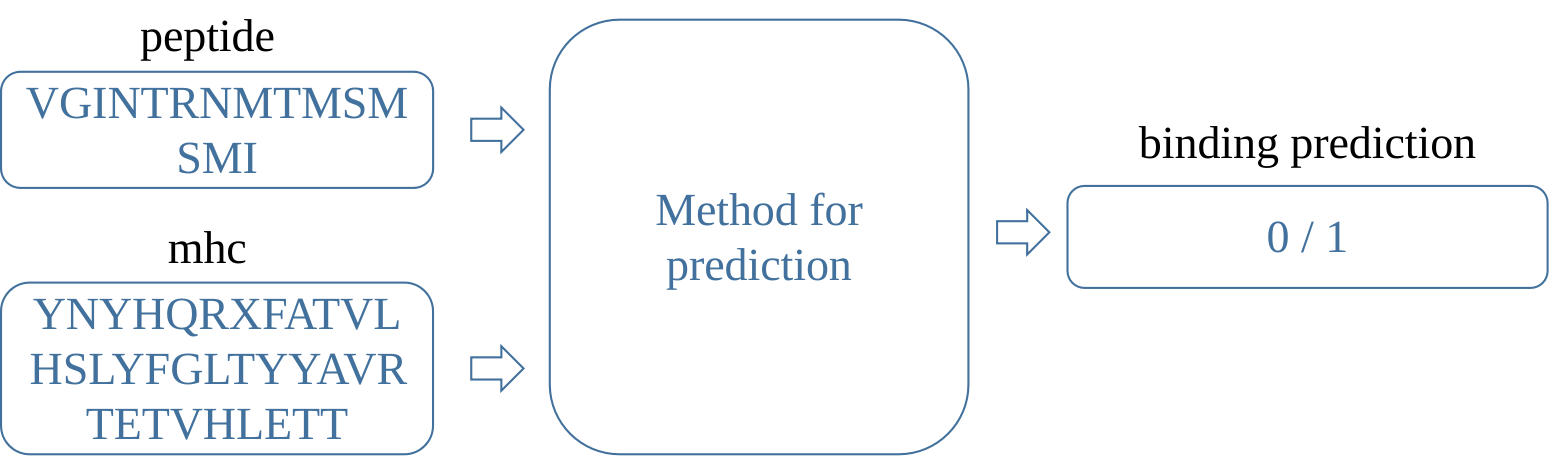
\includegraphics[width=0.97\textwidth]{img/neoantigen/problem}
			\caption{pMHC binding prediction problem.}
		\end{figure}
\end{frame}
%-------------------------------------------------------
%-------------------------------------------------------


%-------------------------------------------------------
%-------------------------------------------------------
%\begin{frame}{Objetivos}{}	
%	\begin{figure}
%		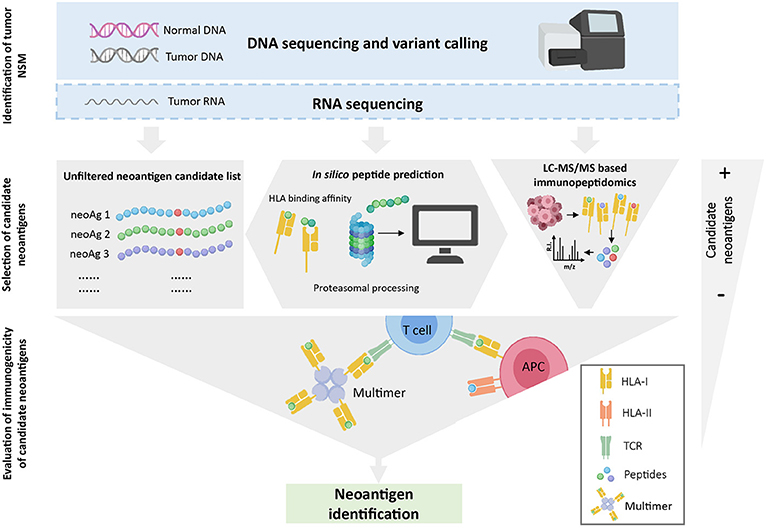
\includegraphics[width=0.97\textwidth]{img/neoantigen/pipeline_neoantigen}
		%\caption{Proceso de la detección de neo antígenos \cite{garcia2019determinants}.}
%	\end{figure}
%\end{frame}
%-------------------------------------------------------
%-------------------------------------------------------


%%%%%%%%%%%%%%%%%%%%%%%%%%%%%%%%%%%%%%%%%%%%%%%%%%%%%%%%%%%%%%%%%%%%%%%%%%%%%%%%%%%%%%%%%%%%%%%%%%%%%%%%%%%%%%%%
%%%%%%%%%%%%%%%%%%%%%%%%%%%%%%%%%%%%%%%%%%%%%%%%%%%%%%%%%%%%%%%%%%%%%%%%%%%%%%%%%%%%%%
\section{Related Works}
%%%%%%%%%%%%%%%%%%%%%%%%%%%%%%%%%%%%%%%%%%%%%%%%%%%%%%%%%%%%%%%%%%%%%%%%%%%%%%%%%%%%%%%%%%%%%%%%%%%%%%%%%%%%%%%%
%%%%%%%%%%%%%%%%%%%%%%%%%%%%%%%%%%%%%%%%%%%%%%%%%%%%%%%%%%%%%%%%%%%%%%%%%%%%%%%%%%%%%%


%-------------------------------------------------------
%-------------------------------------------------------
\begin{frame}{Related Works}{Transformers}
	
	\fontsize{8pt}{5pt}\selectfont
	
	\begin{table}[]
		\centering
		\caption{Recent works based on transformers and transfer learning.}		
		\setlength{\tabcolsep}{0.5em} % for the horizontal padding
		{\renewcommand{\arraystretch}{2}% for the vertical padding
			\begin{tabular}{p{0.6cm}p{0.6cm}p{2cm}p{5cm}}
				\textbf{Year} & \textbf{Ref.}                                  & \textbf{Name} & \textbf{Method}                                                                                                                                                                                                         \\ \hline
				2022 		  & \cite{zhang2022hlab} 		  &		\textbf{HLAB} 			 	   & Uses protBert model incascade with a RNN with attention  \\
				2022          & \cite{wang2022mhcroberta}     &     MHCRoBERTa           & Five encoders with 12 multiple-head self-attention pre-trainned with self-supervision             \\
				2022          & \cite{chu2022transformer}     &     \textbf{TransPHLA}             & Based on four modules: an embedding block, an encoder block (multiple self-attention), a feature optimization block (FC layer), and a projection block (FC layer used to predict)          \\
				2021          & \cite{cheng2021bertmhc}       &     BERTMHC             & Uses TAPE model followed by a linear layer.                          \\
				2021          & \cite{gasser2021interpreting} &     ImmunoBERT    	        & The same as BERTMHC focused on MHC-class I  \\
				
				           
			\end{tabular}
		}
	\end{table}	
\end{frame}
%-------------------------------------------------------
%-------------------------------------------------------


%%%%%%%%%%%%%%%%%%%%%%%%%%%%%%%%%%%%%%%%%%%%%%%%%%%%%%%%%%%%%%%%%%%%%%%%%%%%%%%%%%%%%%%%%%%%%%%%%%%%%%%%%%%%%%%%
%%%%%%%%%%%%%%%%%%%%%%%%%%%%%%%%%%%%%%%%%%%%%%%%%%%%%%%%%%%%%%%%%%%%%%%%%%%%%%%%%%%%%%
\section{Proposal}
%%%%%%%%%%%%%%%%%%%%%%%%%%%%%%%%%%%%%%%%%%%%%%%%%%%%%%%%%%%%%%%%%%%%%%%%%%%%%%%%%%%%%%%%%%%%%%%%%%%%%%%%%%%%%%%%
%%%%%%%%%%%%%%%%%%%%%%%%%%%%%%%%%%%%%%%%%%%%%%%%%%%%%%%%%%%%%%%%%%%%%%%%%%%%%%%%%%%%%%



%-------------------------------------------------------
%-------------------------------------------------------
\begin{frame}{Proposal}{}

	\vspace{0.5cm}
	\begin{figure}[H]
		\centering
		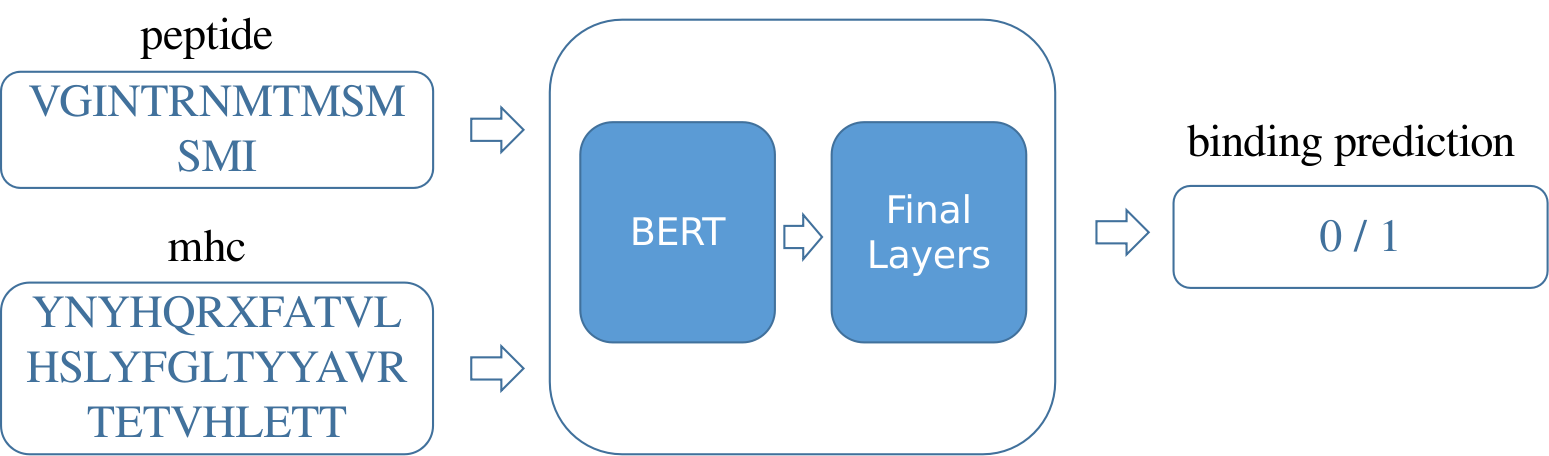
\includegraphics[width=0.9\textwidth]{img/neoantigen/proposal4}	
		\caption{Proposal for pMHC binding and presentation prediction.}
		\label{fig:neo_det_seq}
	\end{figure}
\end{frame}
%-------------------------------------------------------
%-------------------------------------------------------




%%%%%%%%%%%%%%%%%%%%%%%%%%%%%%%%%%%%%%%%%%%%%%%%%%%%%%%%%%%%%%%%%%%%%%%%%%%%%%%%%%%%%%%%%%%%%%%%%%%%%%%%%%%%%%%%
%%%%%%%%%%%%%%%%%%%%%%%%%%%%%%%%%%%%%%%%%%%%%%%%%%%%%%%%%%%%%%%%%%%%%%%%%%%%%%%%%%%%%%
\section{Preliminary Results}
%%%%%%%%%%%%%%%%%%%%%%%%%%%%%%%%%%%%%%%%%%%%%%%%%%%%%%%%%%%%%%%%%%%%%%%%%%%%%%%%%%%%%%%%%%%%%%%%%%%%%%%%%%%%%%%%
%%%%%%%%%%%%%%%%%%%%%%%%%%%%%%%%%%%%%%%%%%%%%%%%%%%%%%%%%%%%%%%%%%%%%%%%%%%%%%%%%%%%%%

%%%%%%%%%%%%%%%%%%%%%%%%%%%%%%%%%%%%%%%%%%%%%%%%%%%%%%%%%%%%%%%%%%%%%%%%%%%%%%%%%%%%%%%%%%%%%%%%%%%%%%%%%%%%%%%%
%%%%%%%%%%%%%%%%%%%%%%%%%%%%%%%%%%%%%%%%%%%%%%%%%%%%%%%%%%%%%%%%%%%%%%%%%%%%%%%%%%%%%%
\subsection{Models and databases}
%%%%%%%%%%%%%%%%%%%%%%%%%%%%%%%%%%%%%%%%%%%%%%%%%%%%%%%%%%%%%%%%%%%%%%%%%%%%%%%%%%%%%%%%%%%%%%%%%%%%%%%%%%%%%%%%
%%%%%%%%%%%%%%%%%%%%%%%%%%%%%%%%%%%%%%%%%%%%%%%%%%%%%%%%%%%%%%%%%%%%%%%%%%%%%%%%%%%%%%

%-------------------------------------------------------
%-------------------------------------------------------
\begin{frame}{Databases}{}
	
We used the dataset from NetMHCIIpan3.2 \cite{jensen2018improved} and HLAB  \cite{zhang2022hlab}.

\begin{table}[h]
	\centering
	\caption{Number of samples used in training, evaluation and testing.}
	\setlength{\tabcolsep}{0.8em} % for the horizontal padding
	{\renewcommand{\arraystretch}{1.3}% for the vertical padding
		
		\begin{tabular}{lll}
			& \textbf{NetMHCIIpan3.2} & \textbf{HLAB} \\ \hline
			\textbf{Train}      & 107424  &   539019   \\
			\textbf{Validation} & 13428  &   179673   \\
			\textbf{Testing}    & 13429  &  172580   
		\end{tabular}
		
	}
\end{table}

\end{frame}
%-------------------------------------------------------
%-------------------------------------------------------

%-------------------------------------------------------
%-------------------------------------------------------
\begin{frame}{Models}{}
	
	We are going to evaluate these BERT models: ESM1-b \cite{rives2021biological}, PortBert \cite{elnaggar2007prottrans}, ESM2 \cite{lin2023evolutionary}, and TAPE \cite{rao2019evaluating}. Moreover, the Bi-LSTM with attention layer is based on HLAB \cite{zhang2022hlab}.
	
	\begin{table}[h]
		\centering
		\caption{Final layers in cascade after the BERT architecture.}
		\setlength{\tabcolsep}{0.8em} % for the horizontal padding
		{\renewcommand{\arraystretch}{1.3}% for the vertical padding
			
			\begin{tabular}{lp{6cm}}
				& \textbf{Description}\\ \hline
				\textbf{LINEAR}      & BERT architecture followed by a linear layer        \\
				\textbf{RNN} & BERT architecture followed by a BiLSTM layer and then a Linear layer        \\
				\textbf{RNN-ATT}    & BERT architecture followed by a BiLSTM layer with attention and then a Linear layer       
			\end{tabular}
			
		}
	\end{table}
	
\end{frame}
%-------------------------------------------------------
%-------------------------------------------------------


%-------------------------------------------------------


%%%%%%%%%%%%%%%%%%%%%%%%%%%%%%%%%%%%%%%%%%%%%%%%%%%%%%%%%%%%%%%%%%%%%%%%%%%%%%%%%%%%%%%%%%%%%%%%%%%%%%%%%%%%%%%%
%%%%%%%%%%%%%%%%%%%%%%%%%%%%%%%%%%%%%%%%%%%%%%%%%%%%%%%%%%%%%%%%%%%%%%%%%%%%%%%%%%%%%%
\subsection{Comparison of LINEAR, RNN and RNN-ATT}
%%%%%%%%%%%%%%%%%%%%%%%%%%%%%%%%%%%%%%%%%%%%%%%%%%%%%%%%%%%%%%%%%%%%%%%%%%%%%%%%%%%%%%%%%%%%%%%%%%%%%%%%%%%%%%%%
%%%%%%%%%%%%%%%%%%%%%%%%%%%%%%%%%%%%%%%%%%%%%%%%%%%%%%%%%%%%%%%%%%%%%%%%%%%%%%%%%%%%%%


\begin{frame}{Training}{ Comparison of LINEAR, RNN and RNN-ATT}
	
	\begin{figure}
		\centering     %%% not \center
		\subfigure[Training in ESM2\_t6\_8M]{\label{fig:a}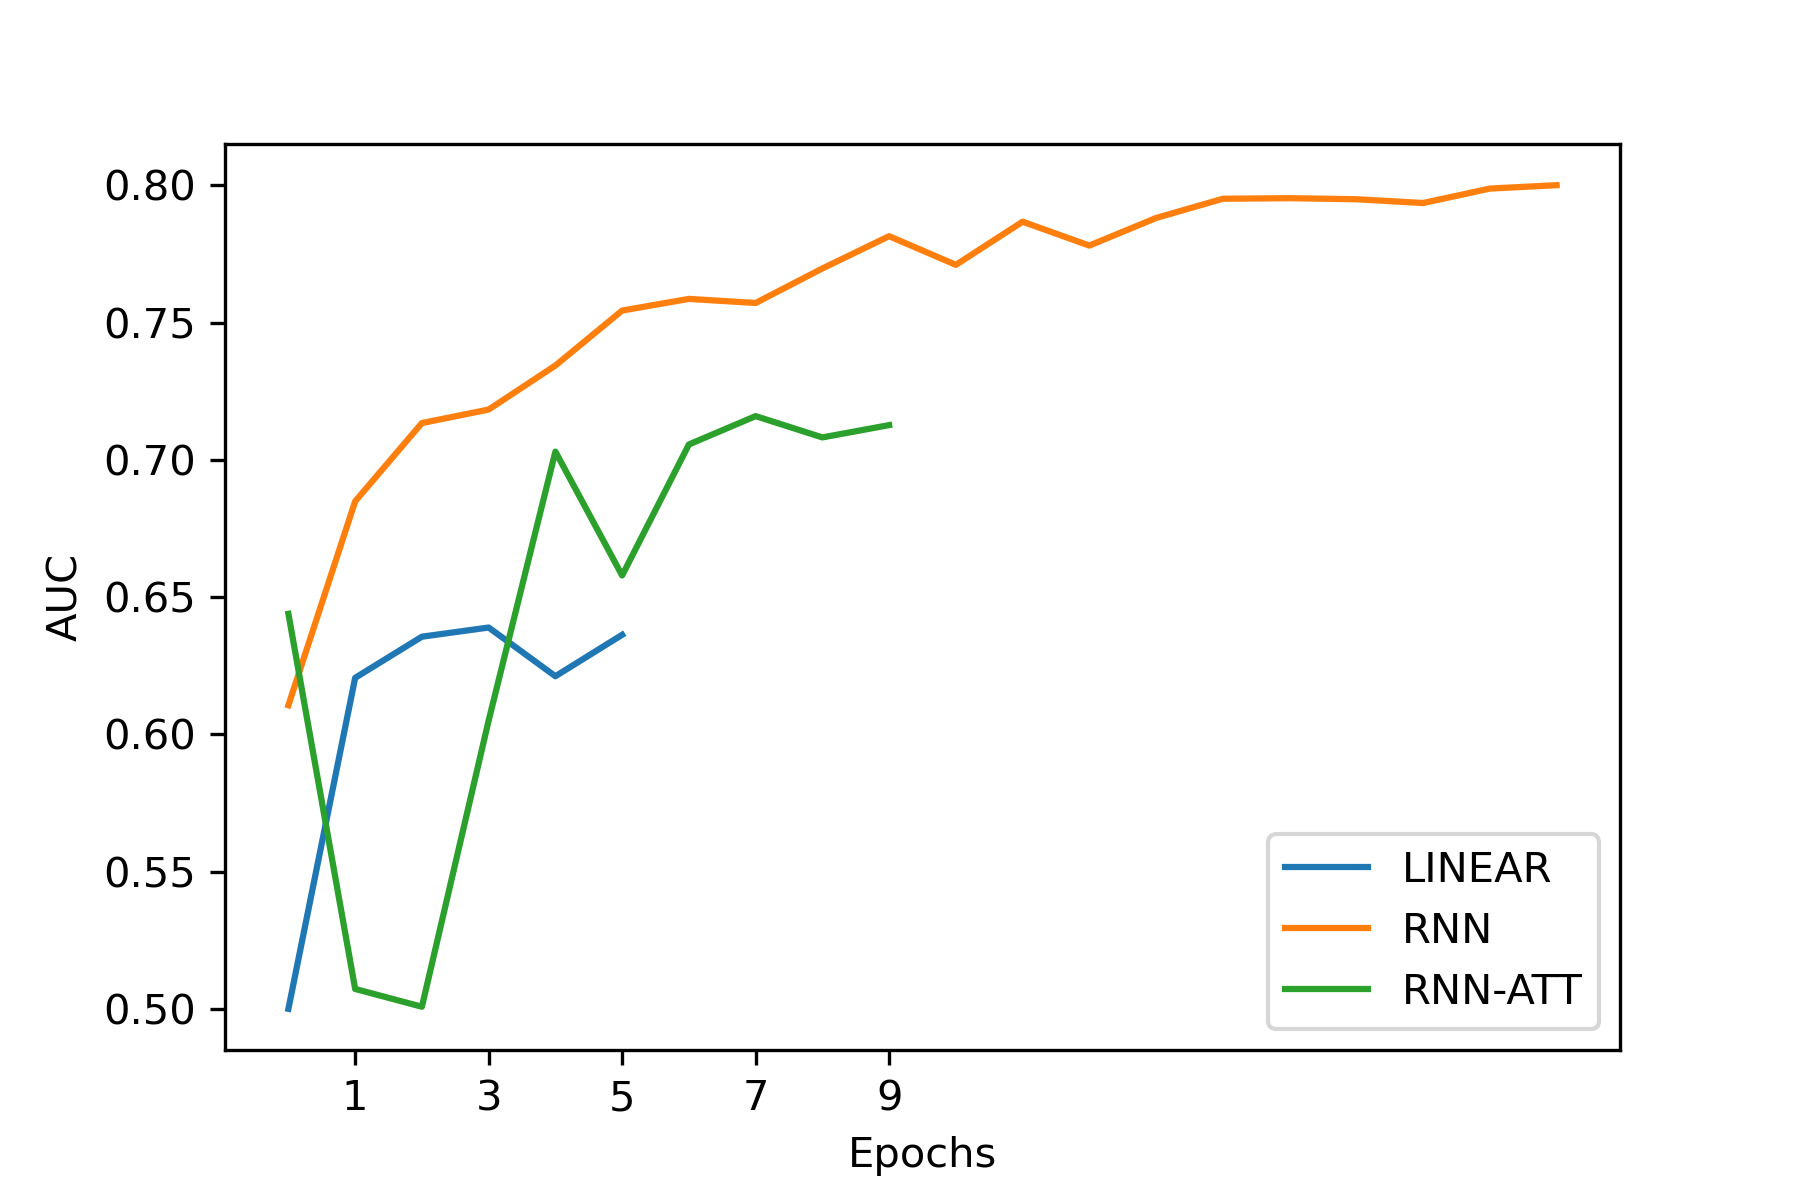
\includegraphics[width=50mm]{img/neoantigen/training_train_1train_2_train_3_}}
		\subfigure[Training in ESM2\_t30\_150M]{\label{fig:b}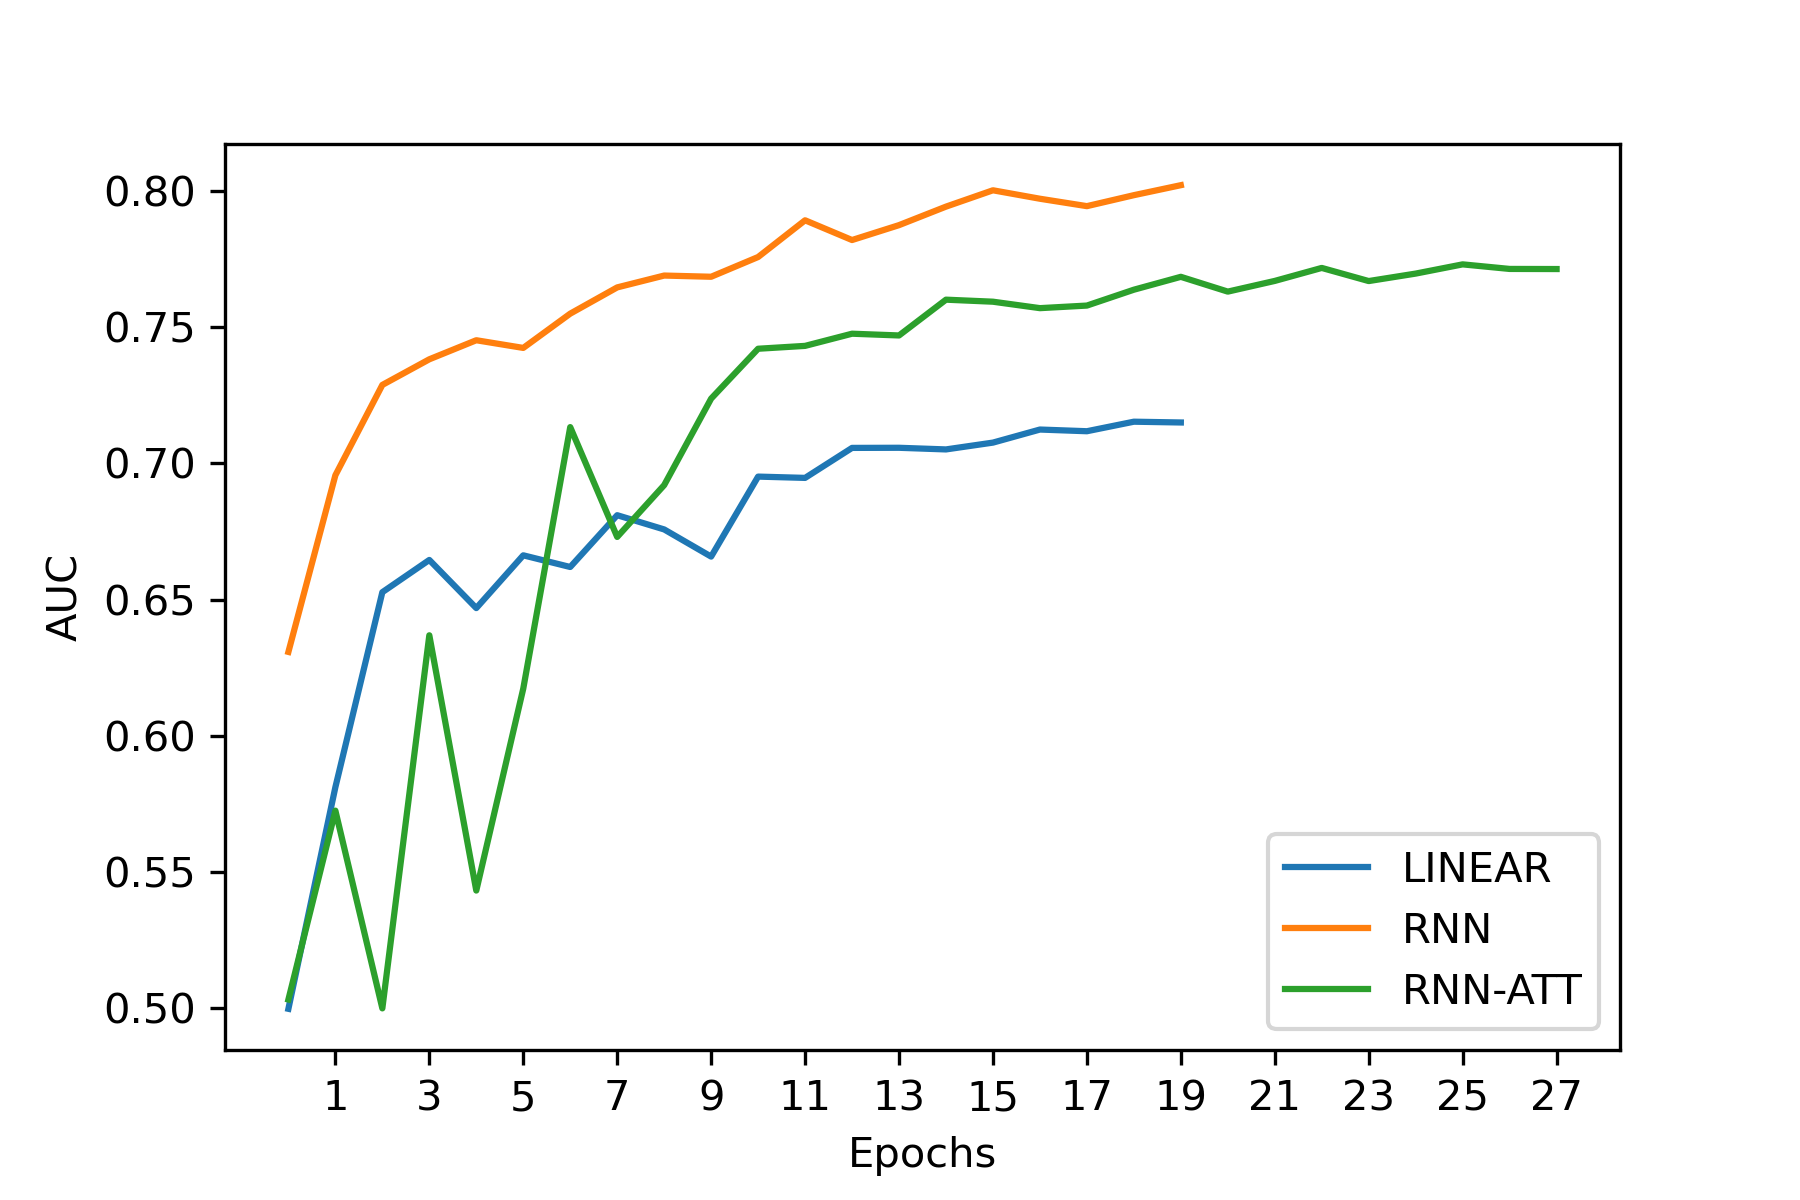
\includegraphics[width=50mm]{img/neoantigen/training_train_7train_8_train_9_}}
		\caption{Training comparison of ESM2 models in NetMHCIIpan3.2 dataset. We used 30 epochs with early stooping.}
	\end{figure}

	
\end{frame}


%-------------------------------------------------------
%-------------------------------------------------------
\begin{frame}{Testing}{Comparison of LINEAR, RNN and RNN-ATT}
	
	\begin{table}[]
		\centering
		\caption{F1-score comparison of ESM2 (BERT model) followed by a LINEAR, RNN and RNN-ATT layers. It was evaluated in NetMHCIIpan3.2 dataset.}
		\setlength{\tabcolsep}{0.8em} % for the horizontal padding
		{\renewcommand{\arraystretch}{1.3}% for the vertical padding
			
		\begin{tabular}{llll}
			Bert Model           & Linear & RNN             & RNN-ATT \\ \hline
			ESM2\_T6\_8M    & nan    & \textbf{0.7679} & 0.6684  \\
			ESM2\_T12\_35M  & 0.6638 & \textbf{0.7734} & 0.7367  \\
			ESM2\_T30\_150M & 0.6709 & \textbf{0.7714} & 0.7363 
		\end{tabular}
	}
	\end{table}
	
\end{frame}
%-------------------------------------------------------

%-------------------------------------------------------
%-------------------------------------------------------
%\begin{frame}{Training}{}

%	\begin{figure}[H]
%		\centering
%		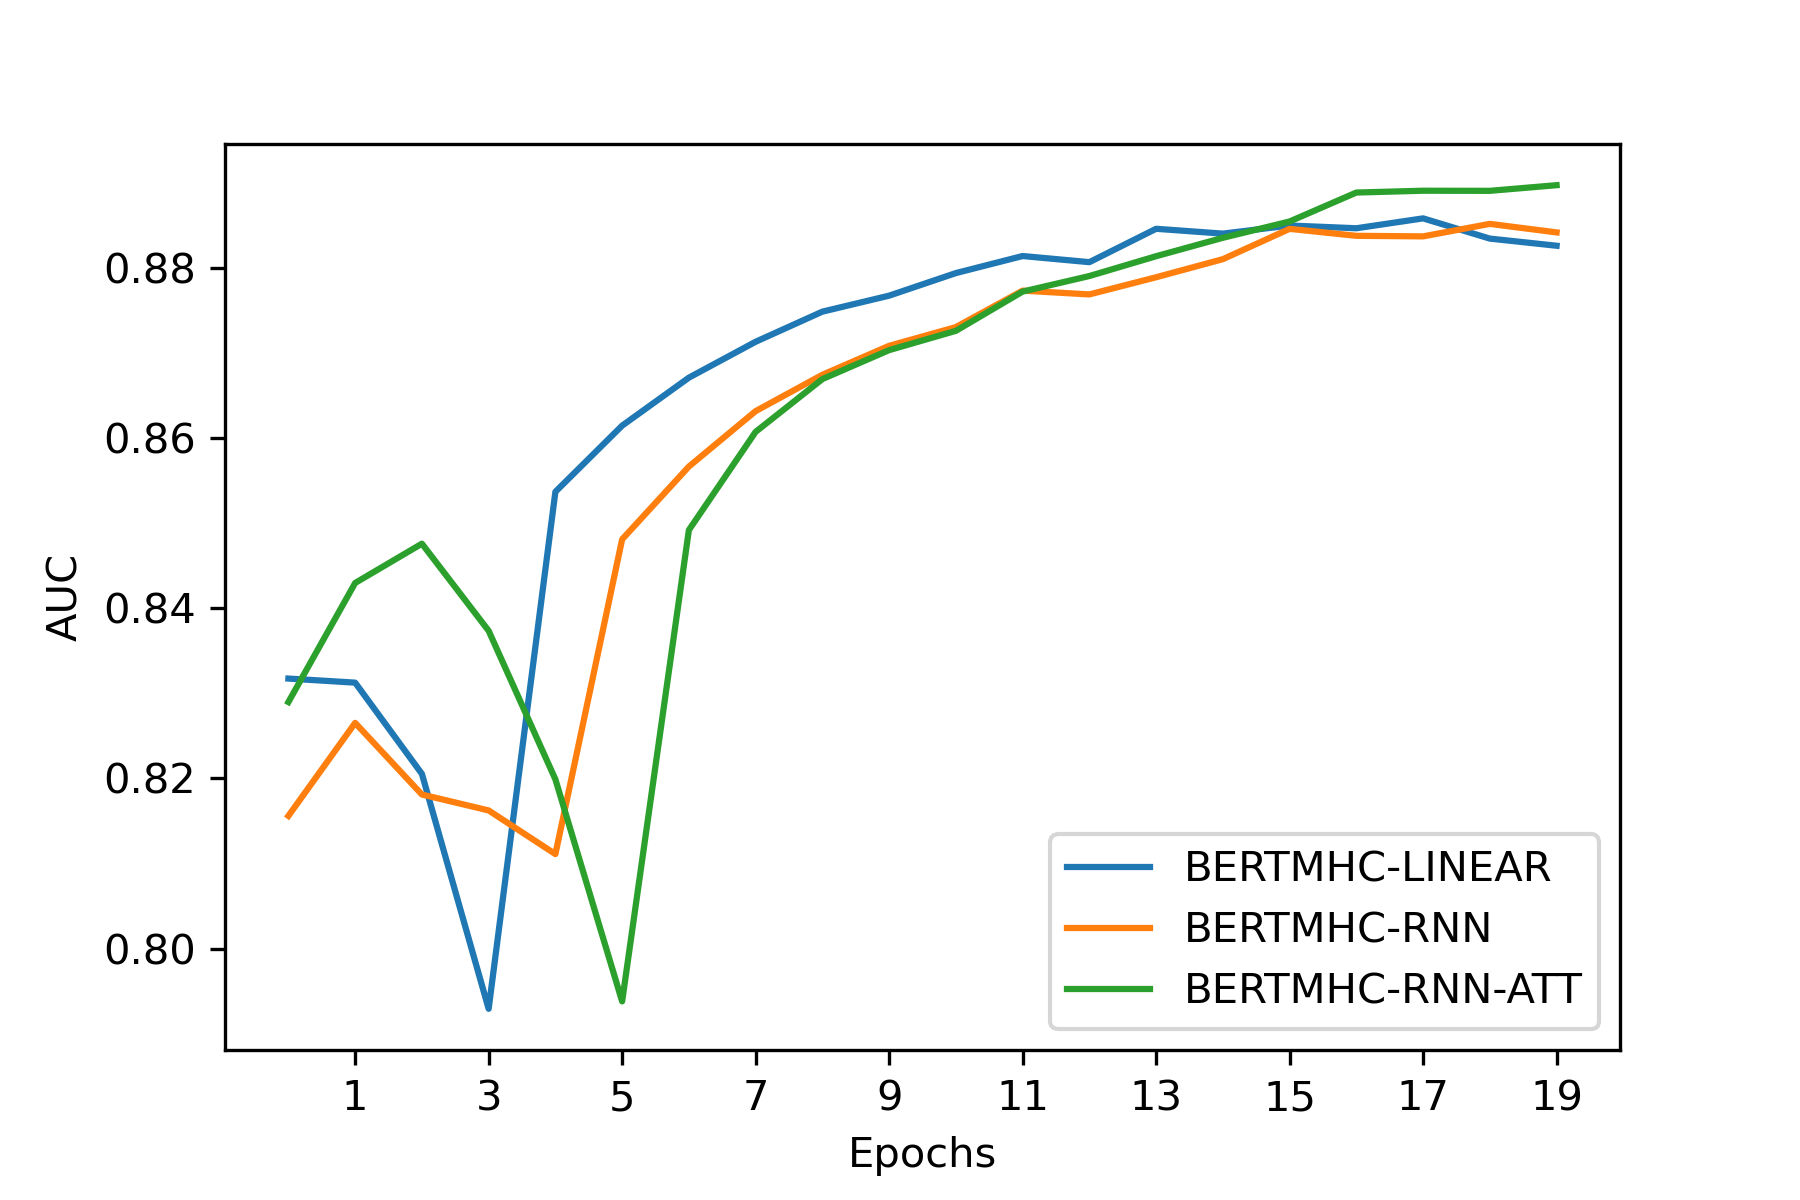
\includegraphics[width=0.8\textwidth]{img/metrics/training_3_7_8}	
%		\caption{AUC per epoch of models.}		
%	\end{figure}
%\end{frame}
%-------------------------------------------------------
%-------------------------------------------------------


%%%%%%%%%%%%%%%%%%%%%%%%%%%%%%%%%%%%%%%%%%%%%%%%%%%%%%%%%%%%%%%%%%%%%%%%%%%%%%%%%%%%%%%%%%%%%%%%%%%%%%%%%%%%%%%%
%%%%%%%%%%%%%%%%%%%%%%%%%%%%%%%%%%%%%%%%%%%%%%%%%%%%%%%%%%%%%%%%%%%%%%%%%%%%%%%%%%%%%%
\subsection{Comparison of pre-trained BERT models}
%%%%%%%%%%%%%%%%%%%%%%%%%%%%%%%%%%%%%%%%%%%%%%%%%%%%%%%%%%%%%%%%%%%%%%%%%%%%%%%%%%%%%%%%%%%%%%%%%%%%%%%%%%%%%%%%
%%%%%%%%%%%%%%%%%%%%%%%%%%%%%%%%%%%%%%%%%%%%%%%%%%%%%%%%%%%%%%%%%%%%%%%%%%%%%%%%%%%%%%

%-------------------------------------------------------
%-------------------------------------------------------
\begin{frame}{Comparison of pre-trained BERT models}{}
		 
		 \begin{table}[]
		 	\centering
		 	\caption{Comparison of pre-trained BERT mpdels: TAPE, ESM2, and PortBert. We trained these models (followed in cascade by RNN layers) in HLAB dataset for three epochs.}
		 	\setlength{\tabcolsep}{0.8em} % for the horizontal padding
		 	{\renewcommand{\arraystretch}{1.3}% for the vertical padding
		 		
		 	
		 	\begin{tabular}{lccccc}
		 		\textbf{Models}       & \textbf{AUC}    & \textbf{Precis.} & \textbf{Recall} & \textbf{F1}     & \textbf{Acc}    \\ \hline
		 		tape\_freeze          & 0.9345          & 0.9283             & 0.9416          & 0.9348          & 0.9345          \\
		 		esm2\_t6      & \textbf{0.9351} & \textbf{0.9253}    & \textbf{0.9464} & \textbf{0.9357} & \textbf{0.9351} \\
		 		esm2\_t12     & 0.9344          & 0.9251    & 0.9451          & 0.9350          & 0.9344          \\
		 		esm2\_t30     & 0.9303          & 0.9185    & 0.9440          & 0.9311          & 0.9303          \\
		 		esm2\_t33     & 0.6816          & 0.7139             & 0.6044          & 0.6546          & 0.6818          \\
		 		protbert\_bfd & 0.9083          & 0.9176             & 0.8968          & 0.9071          & 0.9083          \\
		 		netMHCpan4.1          & 0.9006          & \textbf{0.9586}    & 0.8372          & 0.8938          & 0.9007         
		 	\end{tabular}
	 	
	 	}
		 \end{table}
	
\end{frame}
%-------------------------------------------------------
%-------------------------------------------------------

%-------------------------------------------------------
%-------------------------------------------------------
%\begin{frame}{Comparison}{}
	
%\begin{table}[]
%	\caption{Metrics comparison of BERTMHC-LINEAR, BERTMHC-RNN and BERTMHC-RNN-ATT}
%	\setlength{\tabcolsep}{0.8em} % for the horizontal padding
%	{\renewcommand{\arraystretch}{1.3}% for the vertical padding
%	\begin{tabular}{llllll}
%		\textbf{Model} & \textbf{Acc} & \textbf{Precision} & \textbf{Recall} & \textbf{Fscore} & \textbf{AUC} \\ \hline
%		LINEAR & 0.8070       & 0.8012             & \textbf{0.8005}          & \textbf{0.8009}          & \textbf{0.8005}       \\
%		RNN & 0.8023       & 0.7972             & 0.7932          & 0.7949          & 0.7932       \\
%		RNN-ATT & \textbf{0.8086}       & \textbf{0.8082}             & 0.7937          & 0.7985          & 0.7937      
%	\end{tabular}
%}
%\end{table}
%\end{frame}
%-------------------------------------------------------
%-------------------------------------------------------








%%%%%%%%%%%%%%%%%%%%%%%%%%%%%%%%%%%%%%%%%%%%%%%%%%%%%%%%%%%%%%%%%%%%%%%%%%%%%%%%%%%%%%%%%%%%%%%%%%%%%%%%%%%%%%%%
%%%%%%%%%%%%%%%%%%%%%%%%%%%%%%%%%%%%%%%%%%%%%%%%%%%%%%%%%%%%%%%%%%%%%%%%%%%%%%%%%%%%%%
\section{Conclusions}
%%%%%%%%%%%%%%%%%%%%%%%%%%%%%%%%%%%%%%%%%%%%%%%%%%%%%%%%%%%%%%%%%%%%%%%%%%%%%%%%%%%%%%%%%%%%%%%%%%%%%%%%%%%%%%%%
%%%%%%%%%%%%%%%%%%%%%%%%%%%%%%%%%%%%%%%%%%%%%%%%%%%%%%%%%%%%%%%%%%%%%%%%%%%%%%%%%%%%%%


%-------------------------------------------------------
%-------------------------------------------------------
\begin{frame}{Conclusions}{}
	
	\begin{block}{}
		We compared the performance of \textbf{LINEAR, RNN and RNN-ATT} layers in cascade after ESM2 model trained in NetMHCIIpan3.2 dataset (107424 samples). This experiment shows how the \textbf{RNN layer (BiLSTM) outperformed the others}.
	\end{block}

	\begin{block}{}
		Then, we compared \textbf{ESM2, TAPE, and ProtBert} models followed by RNN layers. In this case, we trained the models in the HLAB dataset (539019 samples). from these experiment, \textbf{ESM2\_t6\_8M outperformed other models and even NetMHCpan4.1}. It is important to clarify that we froze the BERT architecture to accelerate the training.
	\end{block}

\end{frame}
%-------------------------------------------------------
%-------------------------------------------------------


%-------------------------------------------------------
%-------------------------------------------------------
\begin{frame}[allowframebreaks]
	\frametitle{References}
	%\bibliographystyle{amsalpha}
	\bibliographystyle{IEEEtran}
	\bibliography{Bibliography.bib}
\end{frame}
%-------------------------------------------------------
%-------------------------------------------------------

%-------------------------------------------------------
%-------------------------------------------------------
\if\mycmd1 % MY THEME
\1{
	{\1
		\begin{frame}[plain,noframenumbering]
			%\finalpage{Thank you}
			\begin{figure}[]
				\centering
				
\includegraphics[width=\textwidth,height=0.7\textheight,keepaspectratio]{img/question.png}
				%\label{img:mot2}
				%\caption{Image example in 2 gray levels.}
			\end{figure}
	\end{frame}}
	\else % CS THEME
	\begin{frame}{Questions?}
		\begin{figure}[]
			\centering
			
\includegraphics[width=\textwidth,height=0.7\textheight,keepaspectratio]{img/question.png}
			%\label{img:mot2}
			%\caption{Image example in 2 gray levels.}
		\end{figure}
		
	\end{frame}
	\fi
	%-------------------------------------------------------
	%-------------------------------------------------------
	

\end{document}